\begin{fig}
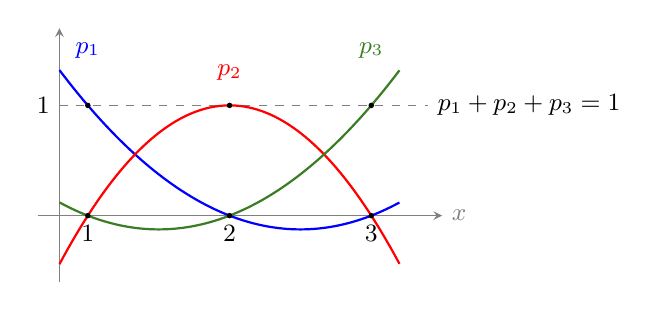
\begin{tikzpicture}[x=1.8cm,y=1.4cm,>=stealth,font=\small]
\draw[->,gray](.65,0)--(3.5,0)node[right]{$x$};\draw[->,gray](.8,-.6)--(.8,1.7);
\draw[gray,dashed](.8,1)--(3.4,1)node[right,text=black]{$p_1+p_2+p_3=1$};
\draw[blue,thick,domain=.8:3.2,samples=80]plot(\x,{(\x-2)*(\x-3)/2});
\draw[red,thick,domain=.8:3.2,samples=80]plot(\x,{-(\x-1)*(\x-3)});
\draw[OliveGreen,thick,domain=.8:3.2,samples=80]plot(\x,{(\x-1)*(\x-2)/2});
\foreach \x in{1,2,3}{\node[below]at(\x,0){$\x$};\fill(\x,1)circle(1pt);\fill(\x,0)circle(1pt);}
\node[blue]at(1,1.5){$p_1$};\node[red]at(2,1.3){$p_2$};\node[OliveGreen]at(3,1.5){$p_3$};
\node[left]at(.8,1){$1$};
\end{tikzpicture}
\figcap{For $\lambda_1=1,\lambda_2=2,\lambda_3=3$, each polynomial is $1$ at its corresponding eigenvalue and $0$ at the other two. Their sum is $1$ everywhere. Substituting $T$ therefore decomposes $v=\sum_jp_j(T)v$ into eigenspace components.}
\end{fig}
\begin{example*}[Compute the eigenspace components]
For $A=\left(\begin{smallmatrix}2&1\\1&2\end{smallmatrix}\right)$ over $\mathbb R$, $m_A=(x-1)(x-3)$. Thus $p_1=(3-x)/2$, $p_3=(x-1)/2$.
For $v=(2,0)^{\mathsf T}$,
\[p_1(A)v=\tfrac12\begin{pmatrix}1&-1\\-1&1\end{pmatrix}\begin{pmatrix}2\\0\end{pmatrix}=\begin{pmatrix}1\\-1\end{pmatrix},\qquad
p_3(A)v=\tfrac12\begin{pmatrix}1&1\\1&1\end{pmatrix}\begin{pmatrix}2\\0\end{pmatrix}=\begin{pmatrix}1\\1\end{pmatrix}.
\]
The two outputs add to $v$ and satisfy $A(1,-1)=(1,-1)$ and $A(1,1)=3(1,1)$. More generally, $p_j(T)$ is identity on its eigenspace and zero on the others, because $p_j(T)u=p_j(\lambda_k)u$ for $u\in E(\lambda_k,T)$. This is the projection onto that eigenspace along the others: it returns exactly that component. Hence $p_j(T)^2=p_j(T)$, $p_i(T)p_j(T)=0$ for $i\ne j$, and $\sum_jp_j(T)=I$.
\end{example*}
